\section{Introducción}
\label{ch:introduccion}

La Programación Lógica Probabilística combina la capacidad deductiva
de la lógica de primer orden con el tratamiento formal de la
probabilidad, lo que la consolida como un paradigma expresivo para
la representación del conocimiento bajo incertidumbre
\cite{deraedt2007problog}. \textit{ProbLog} extiende Prolog con
hechos probabilísticos y calcula la probabilidad de que una consulta
lógica sea verdadera dado un conjunto de evidencias.
    
Los Procesos de Decisión de Markov (MDPs) son el estándar matemático
para modelar agentes que actúan en entornos estocásticos. Formalizados
a mediados del siglo XX con los trabajos de Richard Bellman sobre
programación dinámica \cite{bellman1957dynamic}, los MDPs optimizan
una función de utilidad a lo largo del tiempo. En su formulación
tabular clásica, cada estado del sistema se trata como una entidad
indivisible y las transiciones se almacenan en una tabla que registra
explícitamente la probabilidad de pasar de cada estado a cada otro
bajo cada acción posible. El tamaño de esa tabla crece de forma
exponencial con el número de variables de estado, un fenómeno que
Bellman denominó la ``maldición de la dimensionalidad''
\cite{bellman1957dynamic}. Esta característica hace que la
especificación y la resolución de MDPs se vuelvan costosas conforme
crece la complejidad del dominio \cite{puterman2014markov}.

Bueno et al. propusieron \textbf{MDP-ProbLog} \cite{bueno2016mdp},
un framework que codifica estados, acciones y recompensas dentro de
la sintaxis de la programación lógica y representa MDPs de horizonte
infinito de forma relacional y compacta. Estos problemas de decisión
secuencial no tienen un punto de terminación predefinido; el agente
busca una estrategia óptima a largo plazo. En lugar de tratar cada
estado como una entidad indivisible, MDP-ProbLog adopta una
representación factorizada en la que descompone el estado global en
un conjunto de variables independientes denominadas \textit{fluentes},
de modo que la dinámica del sistema se describe en términos de cómo
cambia cada variable individual. Esta representación hace compacta y
legible la especificación del MDP, aunque la resolución con el
algoritmo de iteración de valor sigue siendo enumerativa y sujeta a
la explosión combinatoria del espacio de estados.

\clearpage

\subsection{Antecedentes}
\label{sec:antecedentes}

La idea de utilizar lenguajes declarativos para especificar MDPs no surge con
MDP-ProbLog. Boutilier, Dean y Hanks \cite{boutilier1999decision} propusieron
a finales de la década de 1990 representaciones factorizadas para abordar la
maldición de la dimensionalidad, con redes bayesianas dinámicas en lugar de
tablas monolíticas para describir las transiciones de estado. Posteriormente,
SPUDD \cite{hoey1999spudd} explotó diagramas de decisión algebraicos para
resolver MDPs factorizados de manera simbólica. Ambas herramientas avanzaron en la especificación compacta de MDPs en los que cada variable de estado solo podía tomar dos valores. El dominio \textit{Factory}, introducido
en la evaluación de SPUDD, precisa este problema. En este escenario se requieren variables categóricas 
ternarias para modelar con precisión el entorno. Para sobreponerse a la limitación, la herramienta los
codifica en don bits, dejando una combinación sin correspondencia física.

\begin{table}[H]
\centering
\caption{Codificación binaria forzada para una variable ternaria en el dominio \textit{Factory}.}
\label{tab:spudd-espurios}
\small
\begin{tabular}{cc|l}
\toprule
\textbf{Bit 1} & \textbf{Bit 2} & \textbf{Calidad de la pintura} \\
\midrule
0 & 0 & Buena (\textit{good}) \\
0 & 1 & Deficiente (\textit{poor}) \\
1 & 0 & Inexistente (\textit{false}) \\
1 & 1 & Estado espurio (\textit{unreachable state}) \\
\bottomrule
\end{tabular}
\end{table}

En el contexto de la Programación Lógica Probabilística, Nitti, Belle y De
Raedt \cite{nitti2016planning} demostraron que los lenguajes probabilísticos
basados en lógica podían servir como especificación declarativa de problemas
de planificación para dominios tanto discretos como continuos. MDP-ProbLog
\cite{bueno2016mdp} se inscribe en esta línea, codifica MDPs de horizonte infinito de manera declarativa dentro de la sintaxis de ProbLog y sustituye el muestreo por inferencia exacta usando Conteo de Modelos Ponderados.

MDP-ProbLog ha sido adoptado como base tecnológica por el equipo de
investigación liderado por el Dr. Héctor Hugo Avilés-Arriaga en la
Universidad Politécnica de Victoria para el desarrollo de sistemas de
navegación y toma de decisiones para vehículos autónomos
\cite{Avilés31122024}. El framework, sin embargo, restringe todos los
fluentes de estado a variables binarias (variables de Bernoulli
independientes), lo que obliga al modelador a representar con predicados
booleanos las variables que el dominio describe de forma natural con más
de dos valores.

\subsection{Definición del Problema}
\label{sec:problema}

MDP-ProbLog carece de un mecanismo nativo para representar variables de
estado con más de dos valores mutuamente excluyentes. Cada fluente se
trata como una variable de Bernoulli independiente. Representar una
variable multivaluada exige descomponerla en un conjunto de predicados
booleanos cuyas combinaciones codifiquen los valores posibles.

El dominio de navegación en cuadrícula, canónico en la literatura de
MDPs \cite{mitchell1997machine, sutton2018reinforcement}, concretiza
esta restricción. Un agente se desplaza desde una posición inicial hasta
una celda meta seleccionando, en cada paso, una de cuatro acciones de
movimiento. La posición del agente forma parte del estado del sistema;
la fila y la columna que ocupa la determinan por completo. Cada
coordenada toma más de dos valores, por lo que no puede representarse
como un único fluente booleano y su codificación exige varios predicados
binarios.

En un grid de $2 \times 3$ con seis celdas, dos fluentes booleanos
producen solo $2^2 = 4$ combinaciones, insuficientes para distinguir
los seis estados. Tres fluentes producen $2^3 = 8$ combinaciones, de
las cuales solo seis corresponden a celdas reales.

La Tabla~\ref{tab:codificacion-binaria-intro} registra la asignación
resultante. Las dos combinaciones sobrantes carecen de correspondencia
física en el dominio. A lo largo del documento se denominan
\textit{estados espurios}.

\begin{table}[H]
    \centering
    \caption{Codificación binaria de las 6 celdas de un grid de $2 \times 3$.}
    \label{tab:codificacion-binaria-intro}
    \small
    \begin{tabular}{ccc|l}
        \toprule
        $b_1$ & $b_2$ & $b_3$ & \textbf{Celda asignada} \\
        \midrule
        0 & 0 & 0 & Celda (1,1) \\
        0 & 0 & 1 & Celda (1,2) \\
        0 & 1 & 0 & Celda (1,3) \\
        0 & 1 & 1 & (sin correspondencia) \\
        1 & 0 & 0 & Celda (2,1) \\
        1 & 0 & 1 & Celda (2,2) \\
        1 & 1 & 0 & Celda (2,3) \\
        1 & 1 & 1 & (sin correspondencia) \\
        \bottomrule
    \end{tabular}
\end{table}

La Figura~\ref{fig:grid-binario-intro} contrasta ambas representaciones.
La descripción por fila ($x$) y columna ($y$) genera exactamente seis
estados. La codificación con tres fluentes binarios ($b_1$, $b_2$,
$b_3$) produce ocho combinaciones, dos de ellas espurias.

\begin{figure}[htbp]
    \centering
    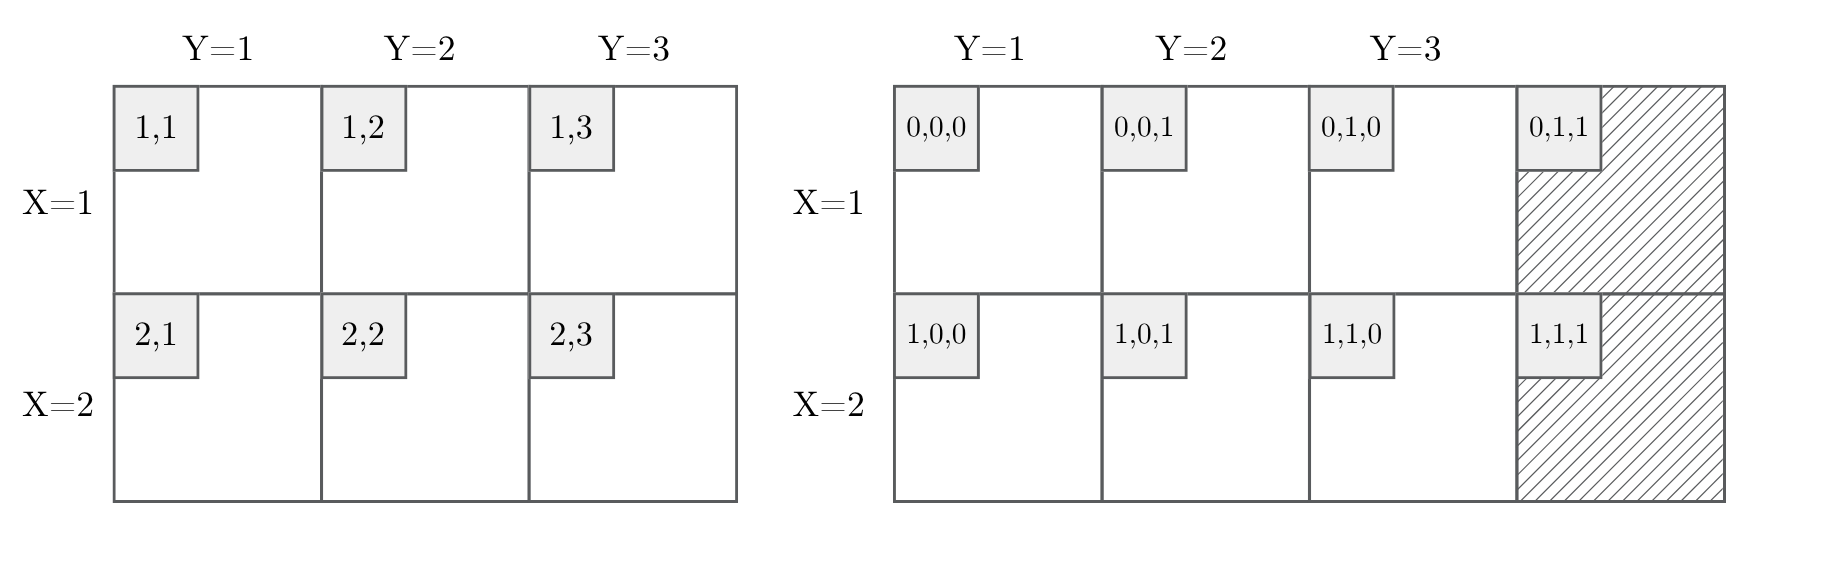
\includegraphics[width=1.0\textwidth]{figuras/2x3_grid_vs_boolean.png}
    \caption{Representación por coordenadas vs. codificación booleana con estados inalcanzables para el grid $2 \times 3$.}
    \label{fig:grid-binario-intro}
\end{figure}

Este desajuste sigue un patrón general. Representar $k$ estados
mutuamente excluyentes requiere $\lceil \log_2(k) \rceil$ fluentes
booleanos, que producen $2^{\lceil \log_2(k) \rceil}$ combinaciones.
Siempre que $k$ no sea potencia exacta de dos, el espacio de estados
contiene combinaciones sin correspondencia física que el modelador debe
gestionar de forma manual. La Tabla~\ref{tab:escalamiento-espurios}
muestra cómo este desajuste crece con el tamaño del dominio.

\begin{table}[H]
    \centering
    \caption{Escalamiento de estados espurios en la codificación binaria por tamaño de grid.}
    \label{tab:escalamiento-espurios}
    \small
    \begin{tabular}{cccccc}
        \toprule
        \textbf{Grid} & \textbf{Celdas ($k$)} & \textbf{Bits necesarios} & \textbf{Combinaciones ($2^{\text{bits}}$)} & \textbf{Espurios} \\
        \midrule
        $2 \times 3$ & 6   & 3 & 8   & 2  \\
        $3 \times 3$ & 9   & 4 & 16  & 7  \\
        $4 \times 4$ & 16  & 4 & 16  & 0  \\
        $5 \times 5$ & 25  & 5 & 32  & 7  \\
        $6 \times 6$ & 36  & 6 & 64  & 28 \\
        \bottomrule
    \end{tabular}
\end{table}

En un grid de $6 \times 6$, 28 de las 64 combinaciones son espurias.
Casi la mitad del espacio de estados no corresponde a ningún escenario
físico del dominio.

La restricción afecta a cualquier dominio con variables categóricas.
El estado de un semáforo, el carril que ocupa un vehículo y la fase
de un proceso manufacturero son variables que admiten más de dos
valores y que MDP-ProbLog obliga a codificar en bits.

El usuario debe gestionar de forma manual las restricciones que impiden
combinaciones sin significado. Sin esa gestión, el algoritmo de
iteración de valor recorre configuraciones inalcanzables y desperdicia
ciclos de cómputo en estados que no contribuyen a la política resultante.

En síntesis, la representación exclusivamente booleana produce modelos
más costosos de escribir para el modelador y menos eficientes de
resolver para el motor. El dominio no puede describirse en sus propios
términos y debe adaptarse a las limitaciones de la herramienta.

\subsection{Objetivos}
\label{sec:objetivos}

\subsubsection{Objetivo General}
\label{subsec:objetivo_general}

Diseñar e integrar soporte para fluentes de estado multivaluados en el núcleo del framework MDP-ProbLog con Disyunciones Anotadas (Annotated Disjunctions), con el fin de proveer una sintaxis de modelado más natural, asegurar la consistencia en los procesos de decisión estocásticos y evaluar el impacto computacional derivado de esta nueva expresividad.

\subsubsection{Objetivos Específicos}
\label{subsec:objetivos_especificos}

\begin{itemize}
    \item Analizar la arquitectura interna actual de MDP-ProbLog, identificando los módulos críticos encargados de la gestión del espacio de estados y la inferencia probabilística para determinar los puntos de extensión.
    \item Desarrollar una estructura de datos y adaptar la lógica de instanciación (\textit{grounding}) para procesar fluentes multivaluados frente a los fluentes binarios tradicionales.
    \item Implementar el soporte para Disyunciones Anotadas en la definición de las transiciones de estado, de modo que los valores de cada variable queden mutuamente excluidos por construcción semántica.
    \item Desarrollar herramientas de inspección para examinar las matrices de transición, las tablas de recompensas y el historial de convergencia de los modelos resueltos.
\end{itemize}

\subsection{Justificación}
\label{sec:justificacion}

La extensión representa un paso necesario para la evolución del framework debido a las limitaciones impuestas por el modelado estrictamente binario. En ausencia de variables categóricas nativas, la arquitectura original transfiere al modelador la tarea de restringir matemáticamente el entorno. Es por ello que el usuario debe diseñar y escribir reglas de integridad manuales para evitar que el sistema asigne valores contradictorios a una misma entidad (por ejemplo, evaluar a un agente que ocupa dos posiciones simultáneamente). Esta práctica introduce ruido en el código y oscurece la lógica real del proceso de decisión bajo capas de restricciones artificiales.

La carga de validación se traslada del modelador al motor lógico con las Disyunciones Anotadas, un constructo nativo de la Programación Lógica Probabilística \cite{vennekens2004lpads} que garantiza la exclusión mutua entre los valores de una variable por construcción semántica. El código ProbLog resultante recobra legibilidad; el modelador concentra su esfuerzo en definir la dinámica y las recompensas del entorno, reduce la carga cognitiva, acorta los tiempos de desarrollo y elimina una fuente recurrente de errores de diseño.

Además de las mejoras en la usabilidad, la precisión de esta nueva codificación resuelve parte de las deficiencias en el rendimiento computacional. Durante el proceso de resolución original, el algoritmo de iteración de valor desperdicia ciclos de cómputo en la evaluación de configuraciones inalcanzables e invierte recursos en estados que jamás contribuirán a la política resultante. Cuando el espacio de estados contiene únicamente los escenarios que el dominio contempla, el sistema elimina las configuraciones redundantes introducidas por la codificación booleana. Este ahorro es directamente proporcional al número de estados espurios evitados y se acumula en dominios con múltiples variables categóricas.

Finalmente, la integración de las Disyunciones Anotadas para modelar fluentes multivaluados no requiere de la modificación de los algoritmos de compilación ni de razonamiento probabilístico. La extensión amplía la expresividad de la herramienta sin comprometer su arquitectura subyacente ni su retrocompatibilidad con los modelos booleanos existentes.


\clearpage

\subsection{Alcances y Limitaciones}
\label{sec:alcances_limitaciones}

\subsubsection{Alcances}
\label{subsec:alcances}

El proyecto abarca el diseño, la implementación y la validación de una
extensión al núcleo del framework MDP-ProbLog que incorpora soporte para
fluentes de estado multivaluados. El desarrollo comprende los siguientes
elementos:

\begin{enumerate}
    \item \textbf{Representación factorizada del espacio de estados.}
    El rediseño de las estructuras de datos necesarias para que el espacio de estados admita factores con más de dos valores posibles y preserva la capacidad de iteración y la indexación eficiente sobre el conjunto completo de estados.

    \item \textbf{Clasificación automática de fluentes.} Se implementó un clasificador que determina automáticamente si un fluente declarado por el usuario es booleano o multivaluado, a partir del análisis de las Disyunciones Anotadas presentes en el programa. El usuario también puede especificar el tipo de forma explícita.

    \item \textbf{Integración con el motor de inferencia.} Se adaptó la interfaz entre MDP-ProbLog y el motor de inferencia de ProbLog para soportar la inyección y el manejo de Disyunciones Anotadas como codificación nativa de los fluentes multivaluados.

    \item \textbf{Adaptación del algoritmo de resolución.} Se reestructuró el flujo de evaluación de transiciones y el algoritmo de Iteración de Valor para operar sobre transiciones agrupadas por factor, de modo que cada variable de estado se evalúa de acuerdo con su cardinalidad real.

    \item \textbf{Herramientas de inspección.} Se desarrollaron utilidades para exportar las matrices de transición, las tablas de recompensas y el historial de convergencia, estas facilitan la verificación y el análisis de los modelos resueltos.

    \item \textbf{Retrocompatibilidad.} La extensión preserva el funcionamiento de los modelos booleanos existentes sin requerir modificaciones por parte del usuario.
\end{enumerate}

La validación funcional se realiza sobre dominios basados en grids, específicamente el grid de Mitchell, un problema canónico en la literatura de MDPs con soluciones óptimas conocidas. En cada dominio se contrastan dos formulaciones del mismo problema, una con codificación booleana y otra con fluentes multivaluados, para evaluar la simplificación del proceso de modelado, la corrección de la política resultante y el comportamiento del solver en términos de convergencia y tamaño del espacio de estados.

\clearpage

\subsubsection{Limitaciones}
\label{subsec:limitaciones}

El desarrollo se restringe a MDPs de horizonte infinito con espacios de estados discretos y completamente observables. Los siguientes puntos delimitan el alcance técnico de la extensión.

\begin{enumerate}
    \item \textbf{Enumeración explícita del espacio de estados.} El alcance de esta extensión se limita a la capa de representación del espacio de estados; la estrategia de resolución enumerativa del framework original permanece sin modificación. El algoritmo de Iteración de Valor continúa recorriendo todos los pares estado-acción en cada iteración, con un costo proporcional al número total de estados por el número de acciones. Dominios con múltiples variables de estado o con variables de cardinalidad alta producen espacios de estados cuya enumeración completa se vuelve computacionalmente costosa.

    \item \textbf{Capa de representación exclusivamente.} El trabajo no modifica los algoritmos de inferencia exacta ni los compiladores de circuitos lógicos utilizados internamente por ProbLog. El efecto de las Disyunciones Anotadas sobre el tamaño de los circuitos compilados es un resultado emergente del compilador subyacente, no una optimización introducida por esta extensión.

    \item \textbf{Convención de declaración de fluentes.} Todos los valores posibles de un fluente multivaluado deben declararse bajo el mismo nombre de predicado. Esta convención habilita la identificación automática de los grupos mutuamente excluyentes, pero impide declarar un fluente cuyos valores se distribuyan entre predicados distintos.

    \item \textbf{Independencia entre variables de estado.} Las reglas de transición del programa deben respetar independencia entre las variables de estado. El sistema evalúa la probabilidad de transición de cada variable por separado y combina los resultados asumiendo que los factores son estocásticamente independientes. Si las reglas del usuario introducen dependencias entre variables que violan este supuesto, el sistema no lo detecta ni emite advertencias.

    \item \textbf{Dominios de evaluación.} Las pruebas se ejecutan sobre dominios de grid discretos de dimensión reducida, seleccionados por la disponibilidad de soluciones de referencia en la literatura. Los resultados no se extrapolan a dominios de gran escala ni a entornos físicos en tiempo real.
\end{enumerate}

El Capítulo~\ref{ch:estado_del_arte} examina los enfoques que fundamentan esta extensión, desde la representación factorizada de MDPs hasta el papel de la Programación Lógica Probabilística en la toma de decisiones secuenciales.